\documentclass[oneside,13pt,a4paper]{report}

% Chargement d'extensions
\usepackage[utf8]{inputenc}
\usepackage[french]{babel}
\usepackage{graphicx}
\usepackage[top=3cm, bottom=3cm, left=3cm, right=3cm]{geometry}
\usepackage{amsmath}
\usepackage{amssymb}

% Commande pour notation 'NB :' (nota bene)
\newcommand\nb[1][0.3]{N\kern-#1emB : }

% csquotes va utiliser la langue définie dans babel
\usepackage[babel=true]{csquotes}

% pour afficher Schéma au lieu de figure dans les legende des images
\addto\captionsfrench{\def\figurename{Schéma}}

% Informations le titre, le(s) auteur(s), la date
\title{Moteur de Requêtes SQL Simples}
\author{
    Belkassim BOUZIDI \and
    Chakib ELHOUITI \and
    Massili KEZZOUL \and
    Ramzi ZEROUAL \and
    Fei YANG
}
\date{\today}


\begin{document}
%\maketitle
\begin{titlepage}
	\centering
	{\scshape\LARGE Universite de Montpellier\par}
	{\scshape\Large Rapport de projet\par}
	\vspace{1.5cm}
	{\huge\bfseries Moteur de requêtes SQL simples\par}
	\vspace{2cm}
	{\Large\itshape
		Massili KEZZOUL \\
		Chakib ELHOUITI \\
		Ramzi ZEROUAL \\
		Belkassim BOUZIDI \\
		Fei YANG \\
		\par}

	\vspace{1.5cm}

	{\Large\itshape
		Encadrante :\par
		Mme. Anne-Muriel \textsc{Chifolleau}
		\par}

	\vspace{2cm}

	\begin{figure}[h]
		\begin{minipage}[c]{.46\linewidth}
			\centering
			
\includegraphics[width=1\textwidth]{img/univ-montpellier.png}
		\end{minipage}
		\hfill%
		\begin{minipage}[c]{.46\linewidth}
			\centering
			
\includegraphics[width=1\textwidth]{img/fds.png}
		\end{minipage}
	\end{figure}

	\par\vspace{1cm}

	\vfill

	% Bottom of the page
	{\large \today\par}
\end{titlepage}




% ------------------------------------- %
% Introduction
% ------------------------------------- %

\parskip=5pt
\chapter*{Introduction}

Dans le cadre du cursus de la Licence 2 informatique, durant notre second semestre, il nous a été proposé un projet qui devra mettre en pratique nos connaissances et nos compétences au travers d'un cahier des charges. L’objet de cette démarche sera d’envisager la conception et le développement d'un moteur d'évaluation de requêtes SQL en mémoire vive.

Les requêtes considérées seront des requêtes simples de la forme : \enquote{SELECT ... FROM ... WHERE ... }  sans imbrication.

À partir d’un ou plusieurs fichiers CSV, Comma-separated Values\footnote{Comma-separated values, format texte ouvert représentant des données tabulaires sous forme de valeurs séparées par des virgules. Voir page \pageref{csv}},
il est demandé de construire une représentation en mémoire des données et d'implémenter les procédures de projection, de sélection et de jointure, découlant de l'interrogation SQL.

Il s'agit principalement de reproduire les fonctionnalités de bases d'un SGBD\footnote{Système de Gestion de Base de Données, voir page \pageref{sgbd}}, tel que MySQL ou bien Oracle.

Notre groupe, composé de cinq personnes : Belkassim Bouzidi, Chakib Elhouiti, Massili Kezzoul, Ramzi Zeroual et Yang Feï, et encadré par Mme Anne-Muriel Chifolleau, a saisie l'opportunité de réaliser ce projet.

\chapter*{Remerciements}
\vspace{\stretch{1}}
\begin{center}

En préambule à ce mémoire nous souhaitons adresser nos remerciements au corps professoral et administratif de la faculté des sciences de Montpellier qui déploient des efforts pour assurer à leurs étudiants une formation actualisée.

En second lieu, nous tenons à remercier notre encadrante Mme:Anne-Muriel Chifolleau pour ses précieux conseils et son aide durant toute la période du travail.

Nos vifs remerciements vont également aux membres du jury pour l’intérêt qu’ils ont porté à notre recherche en acceptant d’examiner notre travail.

Nous remercions Yahia Zeroual pour sa relecture attentive de ce rapport.

\end{center}
\vspace{\stretch{1}}

\parskip=0pt
\tableofcontents

% Espacement entre les paragraphes
\parskip=5pt
% ------------------------------------- %
% Organisation
% ------------------------------------- %

\chapter{Organisation du projet}
\section{Méthodes d’organisation}

Afin de mener à bien le développement du projet, nous avons décidé de travailler un maximum de temps ensemble et de manière très régulière. Nous nous sommes réunis trois à quatre fois par semaine, en vue de faire le point sur l'avancement du projet et de définir les objectifs restant à atteindre.

Ainsi, selon l'état de progression de la conception du moteur de requêtes, nous réalisâmes les tâches en retard durant le week-end pour ne pas cumuler de retard et respecter l'intégralité du cahier des charges.

Toutes les semaines, nous nous sommes réunis avec notre encadrante, Mme Anne-Muriel Chifolleau. Lors de ces réunions, des mises au point relatives au projet, nous furent prodiguées, cela nous a permis de bénéficier de précieux conseils.

\section{Decoupage du projet}

Nous avons découpé la réalisation du projet en trois grandes phases.

\subsection{Phase de modélisation}

Durant cette étape, nous nous sommes réunis pour définir les fonctionnalités demandées par le projet. Notamment séparer les fonctionnalités importantes de celle moins importantes. Nous avons également choisi les outils de travail collaboratifs et les principales technologies utilisées, ainsi qu’une première modélisation du projet.

\subsection{Phase de développement}

Durant cette phase, nous avons commencé à implémenter les différentes fonctionnalités que nous avons modélisées lors de l'étape précédente, toute en améliorant la modélisation au fur et à mesure de l'avancement de notre projet. Nous avons notamment réalisé des tests pour les différents modules afin de s'assurer de leur bon fonctionnement.

\subsection{Finalisation du projet}

Cette étape a consisté en la réalisation des tests finaux afin de s'assurer que le moteur de requêtes fonctionne en toute circonstance et éventuellement corriger les bogues qui peuvent apparaitre.

\section{Outils de collaboration}

Afin de s'organiser, nous avons décidé d'utiliser Git au travers du serveur GitLab hébergé par le service informatique de la faculté. En effet le logiciel libre Git a facilité grandement la collaboration entre nous. Le serveur GitLab quant à lui est fourni gratuitement par le service informatique de la faculté.

En ce qui concerne la rédaction de ce rapport, nous avons utilisé \LaTeX, système de composition de documents créé par Leslie Lamport, pour faciliter la rédaction à plusieurs.

\begin{figure}[h]
	\begin{minipage}[c]{.46\linewidth}
		\centering
		
\includegraphics[width=1\textwidth]{img/gitlab.png}
		\caption{Logo du GitLab}
	\end{minipage}
	\hfill%
	\begin{minipage}[c]{.46\linewidth}
		\centering
		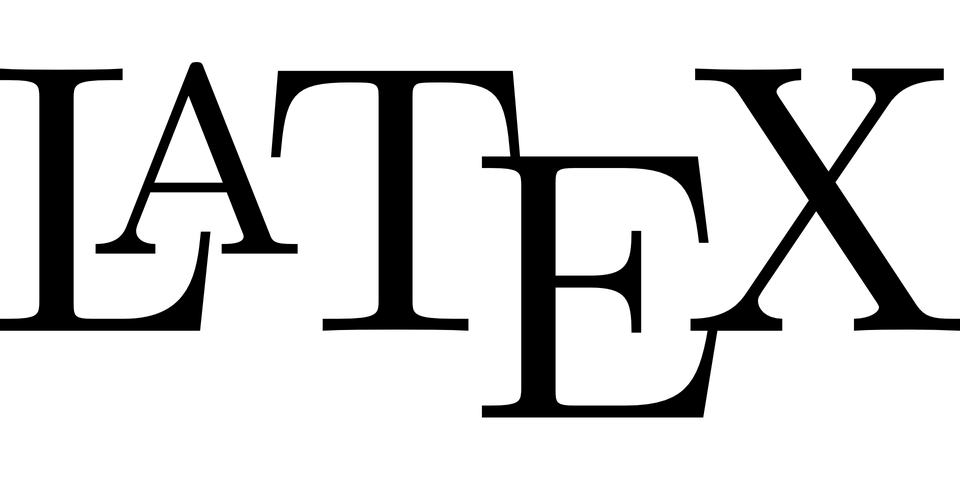
\includegraphics[width=1\textwidth]{img/latex.png}
		\caption{Logo de Latex}
	\end{minipage}
\end{figure}


% ------------------------------------- %
% Le langage SQL
% ------------------------------------- %

\chapter{Le langage SQL et les bases de données}

%Le domaine dans le quelle ce situ notre projet est la gestion d’une base de donnée en utilisant le langage SQL .

%\section{Qu’est-ce qu’une donnée}
\section{Présentation d’une base de donnée}

Une base de données regroupe et stock un ensemble d'informations, qu'on appelle aussi données. En termes simples, les données peuvent êtres des faits liés à tout objet considéré. (Par exemple, un nom, un âge, une taille, un poids ...)

On s'intéresse ici uniquement aux bases de données dites relationnelles, où l'information est organisée dans des tableaux à deux dimensions appelés relations ou tables\footnote{selon le modèle introduit par Edgar F. Codd en 1970.}.
Selon ce modèle relationnel, une base de données consiste en une ou plusieurs relations. Les lignes de ces relations sont appelées des nuplets ou enregistrements. Les colonnes sont appelées des attributs.

\begin{figure}[h]
	\centering
	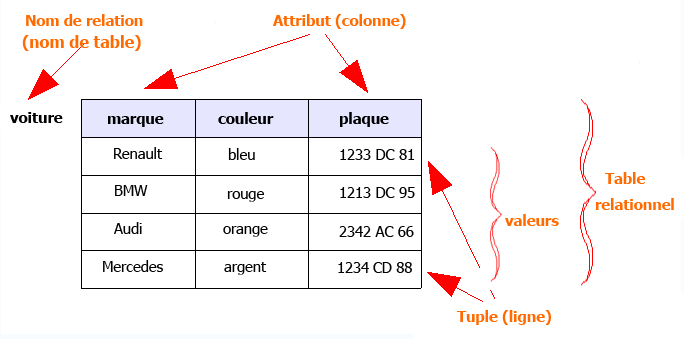
\includegraphics[width=0.7\textwidth]{img/table_relationnel.png}
	\caption{Représentation d'une Table}
\end{figure}

En informatique, une base de données est la pièce centrale des dispositifs de collecte, mise en forme, stockage et utilisation d'informations. Ce dispositif comporte un système de gestion de base de données.

\section{Système de gestion de base de données}
\label{sgbd}

Le système de gestion de base de données (SGBD) est un ensemble de programmes qui permet à ses utilisateurs d'accéder a une base de données, de manipuler des données, ainsi que de contrôler l'accès a la base de données, tout en cachant la complexité des opérations exécutées.

Les SGBD sont utilisés pour de nombreuses applications informatiques, notamment :
\begin{itemize}
	\item les guichets automatiques bancaires
	\item les bibliothèques numérique
	\item les logiciels d'inventaire
	\item et aussi dans de nombreux blogs et sites web.
\end{itemize}

%\vfill

\begin{figure}[h]
	\centering
	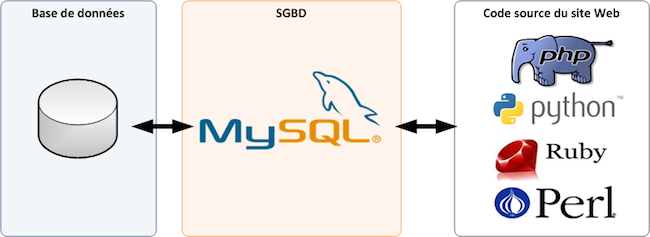
\includegraphics[width=0.7\textwidth]{img/sgbd.png}
	\caption{Représentation d'un SGBD}
\end{figure}

Il existe de nombreux SGBD. En 2008, Oracle détenait près de la moitié du marché avec MySQL et Oracle Database.
Les opérations de recherche et de manipulation des données peuvent être exprimées sous forme de requêtes (anglais query)
dans un langage informatique reconnu par le SGBD. SQL est le langage informatique le plus populaire.

\section{Le langage SQL}
\label{sql}

Le SQL (sigle de Structured Query Language, en français langage de requête structurée) est le langage standard pour traiter les bases de données relationnelles. La programmation SQL peut être utilisée efficacement pour insérer, rechercher, mettre à jour et supprimer des enregistrements de base de données. Les instructions SQL s'écrivent d'une manière qui ressemble à celle de phrases ordinaires en anglais. Cette ressemblance voulue vise à faciliter l'apprentissage et la lecture.

Le SQL est un langage déclaratif, c'est-a-dire qu'il permet de décrire le résultat escompte, sans décrire la manière de l'obtenir. Les SGBD sont équipés d'optimiseurs de requêtes, des mécanismes qui déterminent automatiquement la manière optimale d'effectuer les opérations, notamment par une estimation de la complexité algorithmique.

Le langage SQL est utilisé par des bases de données relationnelles, telles que la base de données MySQL, Oracle, le serveur Ms SQL, Sybase, etc...

Les instructions SQL couvrent 3 principaux domaines :
\begin{itemize}
	\item langage de manipulation de données.
	\item langage de définition de données.
	\item langage de contrôle des données et des transactions.
\end{itemize}
\vspace{0.3cm}

Le domaine considéré dans ce projet est le langage de manipulation de données simples sans imbrication. Exemple de requête SQL : \enquote{SELECT Name FROM Members WHERE Age $ \leq $ 30;}

% -------------------------------------------------------------------------- %
% Présentation du projet : moteur de requêtes SQL simples
% -------------------------------------------------------------------------- %

\chapter{Présentation du projet : moteur de requêtes SQL simples}

\section{Présentation générale}

Notre projet consiste à concevoir et implémenter une application capable de lire des données, exécuter des requêtes SQL simple en mémoire et de renvoyer le résultat. Il s'agit donc de créer une passerelle entre la personne qui exécute la requête SQL et les données. Les difficultés principales sont donc les suivantes :
\vspace{0.3cm}
\begin{itemize}
	\item Savoir charger les données en mémoire;
	\item Savoir interprèter une requête SQL et l'éxecuter sur les données en mémoire;
	\item Savoir retourner le resultat sous un format compréhensible;
\end{itemize}
\vspace{0.3cm}

\section{Les Fonctions Principales}

\subsection{Chargement des données en mémoire}

Les données prises en charge par notre application sont des tables, issues d'une base de données relationnelles, stockées sous forme de fichiers au format CSV.

\subsubsection{Format CSV}
\label{csv}
Comma-separated values, connu sous le sigle CSV, est un format texte ouvert\footnote{format ouvert est défini comme \enquote{tout protocole de communication, d'interconnexion ou d'échange et tout format de données interopérable et dont les spécifications techniques sont publiques et sans restriction d'accès ni de mise en œuvre}} représentant des données tabulaires sous forme de valeurs séparées par des virgules. Ce format n'a jamais vraiment fait l'objet d'une spécification formelle.

Un fichier CSV est un fichier texte, par opposition aux formats dits \enquote{binaires}. Chaque ligne du texte correspond à une ligne du tableau et les virgules correspondent aux séparations entre les colonnes. Les portions de texte séparées par une virgule correspondent ainsi aux contenus des cellules du tableau.

\begin{figure}[!h]
	\centering
	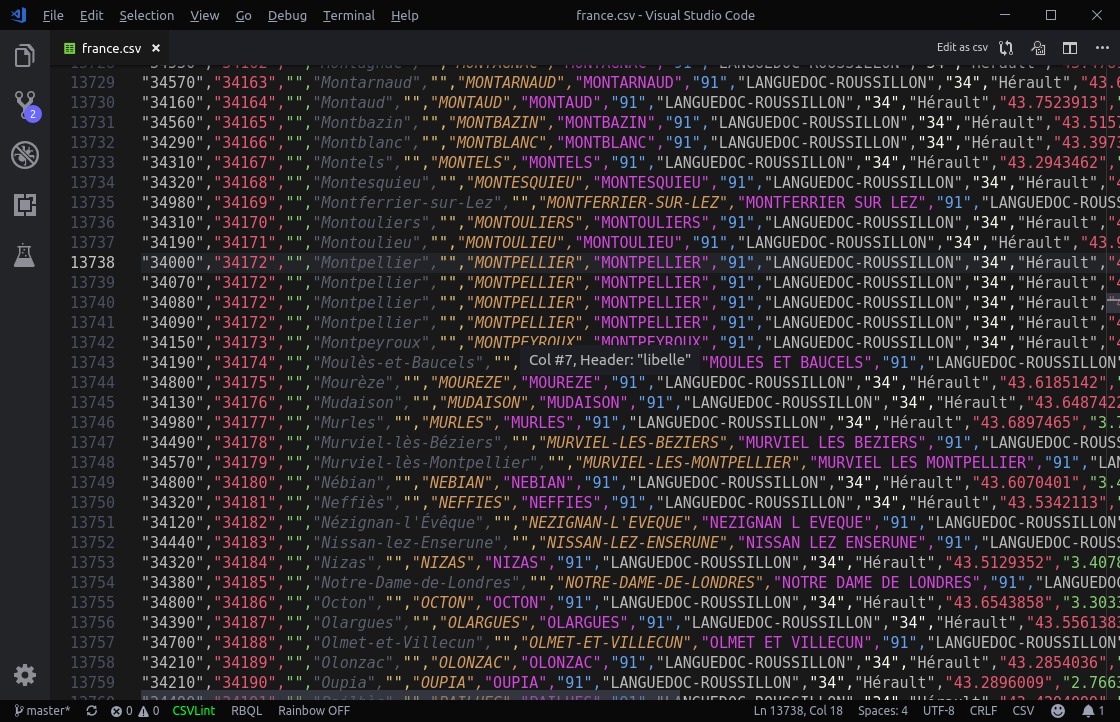
\includegraphics[width=0.85\textwidth]{img/csv.png}
	\caption{Fichier texte sous format CSV}
\end{figure}

\begin{figure}[!h]
	\centering
	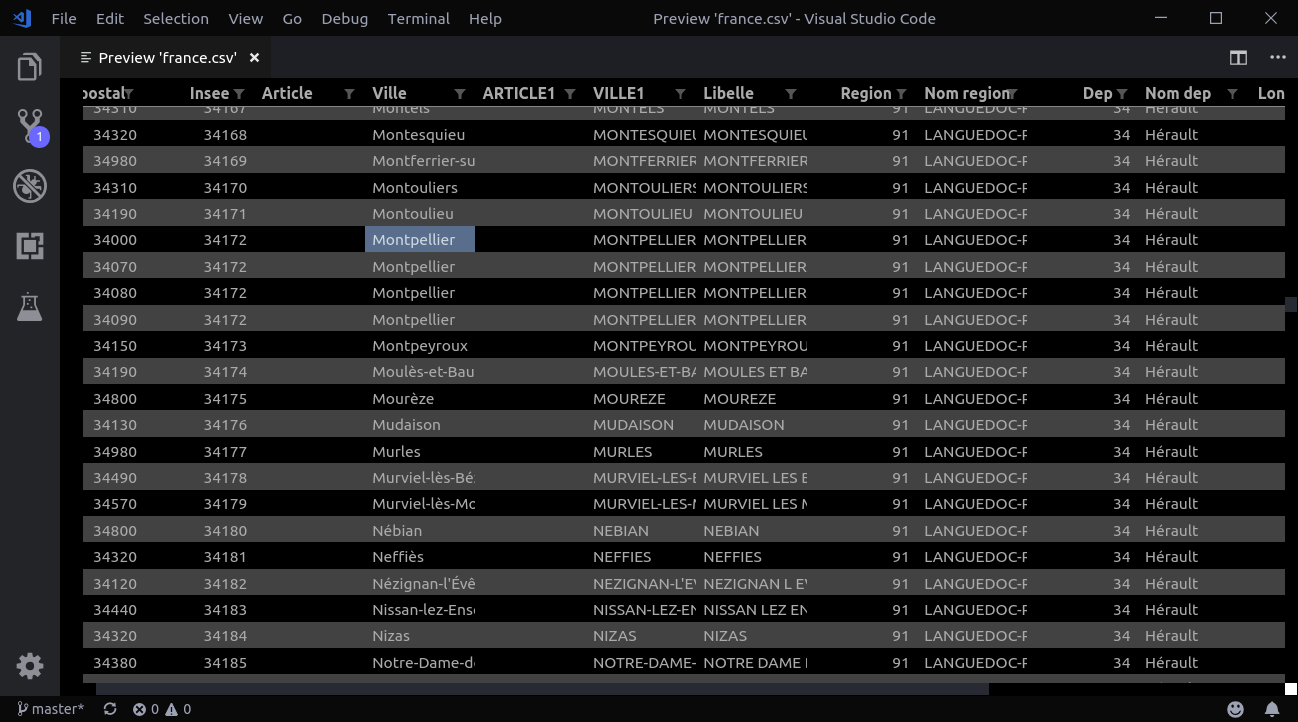
\includegraphics[width=0.85\textwidth]{img/csv_tables.png}
	\caption{Représentation du même fichier en une table de données}
\end{figure}

Les champs texte peuvent également être délimités par des guillemets. Lorsqu'un champ contient lui-même des guillemets, ils sont doublés afin de ne pas être considérés comme début ou fin du champ. Si un champ contient un signe utilise comme séparateur de colonne (virgule, point-virgule, tabulation, etc.), les guillemets sont obligatoires afin que ce signe ne soit pas confondu avec un séparateur.

\subsubsection{Lecture du fichier CSV}

Un fichier CSV est donc un moyen simple de stocker les données d'une base de données.
Ici on considére que :
\begin{itemize}
	\item Le nom du fichier (sans l’extension) est le nom de la table.
	\item La première ligne du fichier ne représente pas des valeurs mais le nom des attributs de la table (c.-à-d. le nom des colonnes).
	\item Toutes les autres lignes représentent des Tuples où chaque valeur est séparée par une virgule.
\end{itemize}
\vspace{0.3cm}

La question qui se pose est donc :
\begin{center}
	\enquote{Comment lire et interpréter un fichier CSV et comment stocker les données qui en résultent ?}
\end{center}

\subsubsection{Lecture de la requête SQL}

Maintenant qu'on a nos tables chargées en mémoire, il faut lire et interpréter la requête SQL\footnote{Structured Query Language: voir Page \pageref{sql}}.

Dans le contexte du projet, les requêtes prisent en charge sont des requêtes SQL simples sans imbrication. Elles respecteront donc la forme suivante :

\enquote{SELECT nomAttribut1,nomAttribut2 FROM nomTable1,nomTable2 WHERE condition1 AND condition2 OR condition3}

Tel que :
\begin{itemize}
	\item Le nom des attributs peut être remplacé par '*', ce qui signifie dans ce cas : \enquote{Tout les attributs};
	\item Il faut spécifier au moins une table (dans le FROM);
	\item Les conditions de sélection (le WHERE) sont facultatives;
\end{itemize}
\vspace{0.3cm}


\subsection{Exécution de la requête SQL}

La dernière étape consiste à exécuter la requête SQL, précédemment interprétée, sur les données chargées en mémoire. On peut clairement découper la requête SQL en trois étapes :

\subsubsection{La projection}

La projection, ou sélection verticale, d'une table sur certaines de ses colonnes est une opération qui fournit une autre table ne contenant qu'un sous-ensemble des colonnes de la table initiale.

Soit la table "FRANCE" suivante :

\begin{tabular}{|l|c|r|}
	\hline
	ville   & region        & codepostal
	\\
	\hline
	Paris01 & Ile-de-france & 75101      \\
	Paris02 & Ile-de-france & 75102      \\
	Paris03 & Ile-de-france & 75103      \\
	\hline
\end{tabular}

La sélection de la colonne ville et code postal se fait par l'instruction :

\enquote{Select ville,codepostal from FRANCE;}

\begin{tabular}{|l|r|}
	\hline
	ville   & codepostal
	\\
	\hline
	Paris01 & 75101      \\
	Paris02 & 75102      \\
	Paris03 & 75103      \\
	\hline
\end{tabular}

\subsubsection{La sélection }

La sélection (sélection horizontale) permet de ne conserver que les tuples qui respectent une condition définie sur les valeurs des attributs, car le but d'une requête SQL est d'extraire des informations spécifiques dans des bases de données,

La sélection permet :
\begin{itemize}
	\item L'affichage de certaines lignes qui vérifient un critère donné ;
	\item Le critère est une expression booleenne plus ou moins compliquée ;
	\item Les conditions de sélection sont données juste après le mot clé WHERE ;
	\item Les conditions sont séparées par des opérateurs logiques, AND et OR ;
\end{itemize}
\pagebreak

Exemple de sélection :

soit la requête SQL suivante :

\begin{center}
	\enquote{SELECT * FROM Employés WHERE age $\leq$ 30;}
\end{center}

Et la table :
\begin{figure}[h]
	\begin{minipage}[c]{.46\linewidth}
		\centering
		\caption{Table 'Employés'}
		%\vspace{0.1cm}
		\begin{tabular}{|l|c|c|r|}
			\hline
			id & nom  & age & idDep
			\\
			\hline
			01 & Emp1 & 30  & 01    \\
			02 & Emp2 & 31  & 01    \\
			03 & Emp3 & 29  & 02    \\
			\hline
		\end{tabular}
	\end{minipage}
	\hfill%
	\begin{minipage}[c]{.46\linewidth}
		\centering
		\caption{Résultat de la sélection}
		\vspace{0.1cm}
		\begin{tabular}{|l|c|c|r|}
			\hline
			id & nom  & age & idDep
			\\
			\hline
			01 & Emp1 & 30  & 01    \\
			03 & Emp3 & 29  & 02    \\
			\hline
		\end{tabular}
	\end{minipage}
\end{figure}

\subsubsection{La jointure}

La jointure est l'opération permettant d'associer plusieurs tables d'une base de données par le biais d'un lien logique de données entre les différentes tables. Le lien étant vérifié par le biais d'un prédicat se situant dans la clause WHERE. Le résultat de l'opération est une nouvelle table. Les tables sélectionnées sont spécifiées dans la partie FROM de la requête SQL.

La jointure entre une table A et B est une table composée de l'ensemble des couples possibles entre leurs éléments respectant le prédicat.

Un exemple est plus parlant qu'une longue explication, prenons deux table Employés et Départements :

\begin{figure}[h]
	\begin{minipage}[c]{.46\linewidth}
		\centering
		\caption{Table 'Employés'}
		\begin{tabular}{|l|c|c|r|}
			\hline
			id & nom  & age & idDep
			\\
			\hline
			01 & Emp1 & 30  & 01    \\
			02 & Emp2 & 31  & 01    \\
			03 & Emp3 & 29  & 02    \\
			\hline
		\end{tabular}
	\end{minipage}
	\hfill%
	\begin{minipage}[c]{.46\linewidth}
		\centering
		\caption{Table 'Départements'}
		\begin{tabular}{|l|c|c|r|}
			\hline
			idDep & nom  & localisation
			\\
			\hline
			01    & Dep1 & Montpellier  \\
			02    & Dep2 & Paris        \\
			\hline
		\end{tabular}
	\end{minipage}
\end{figure}

\enquote{SELECT * FROM Employés,Départements WHERE Employés.idDep = Départements.idDep}

\begin{figure}[h]
	\centering
	\caption{Execution de la jointure}
	\begin{tabular}{|l|c|c|c|c|r|}
		\hline
		id & nom  & age & idDep & nom  & localisation
		\\
		\hline
		01 & Emp1 & 30  & 01    & Dep1 & Montpellier  \\
		02 & Emp2 & 31  & 01    & Dep1 & Montpellier  \\
		03 & Emp3 & 29  & 02    & Dep2 & Paris        \\
		\hline
	\end{tabular}
\end{figure}


\subsection{Retourner le résultat}

La dernière étape consiste à renvoyer la table résultante de l'exécution de la requête sous un format \textit{réutilisable} et \textit{compréhensible}.

\subsubsection{Réutilisable}

Il est question de stocker les données obtenues dans un fichier, sous un format CSV, pour qu'elles soient sauvegardées et réutilisables par l'application.

\pagebreak

\subsubsection{Compréhensible}

Il s'agit de renvoyer la table de manière qu'elle soit compréhensible par l'utilisateur ; c'est-à-dire en affichant les données sous forme d'un tableau.

\begin{figure}[h!]
	\centering
	\caption{Tableau}
	\vspace{0.1cm}
	\begin{tabular}{|l|c|r|}
		\hline
		id & nom  & prenom
		\\
		\hline
		01 & Nom1 & Prenom1 \\
		02 & Nom2 & Prenom2 \\
		03 & Nom3 & Prenom3 \\
		\hline
	\end{tabular}
\end{figure}

\section{Objectif de l'application}

L'objectif de l'application est résumé dans le schéma suivant :
\begin{figure}[!h]
	\centering
	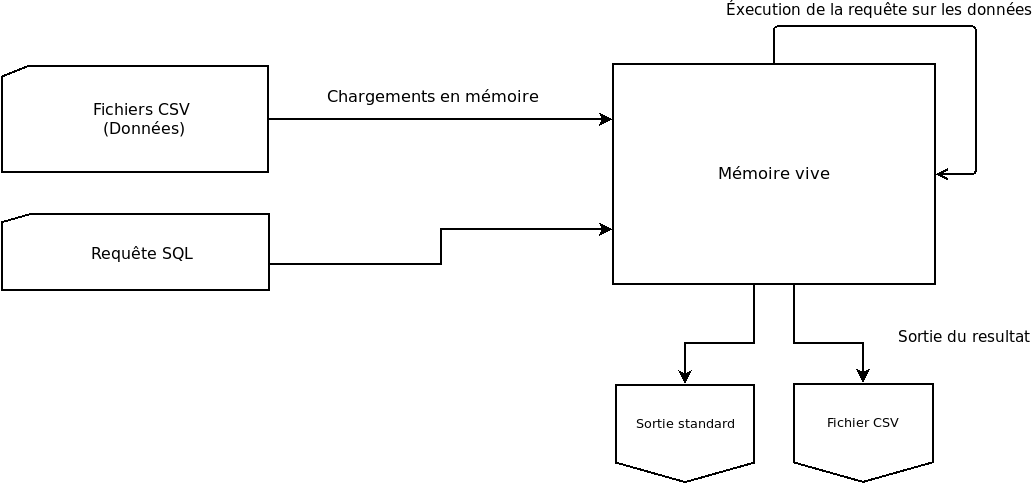
\includegraphics[width=1\textwidth]{img/role_prog.png}
	\vspace{0.1cm}
	\caption{Objectif de l'application}
\end{figure}

% ------------------------------------- %
% Conception du Moteur de Requêtes
% ------------------------------------- %

\chapter{Conception du Moteur de Requêtes}

Nous avons pensé à découper la conception du Moteur de requêtes SQL en deux étapes principales, d'une part comment structurer les données et de l'autre comment gérer la requête SQL.

\section{Structuration des données}

Avant toute chose, il faut commencer par lire les données. Pour cela il faut mettre en \oe uvre une stratégie afin de stocker efficacement les données pour pouvoir y accéder et d’y effectuer les opérations demandées par l'utilisateur, le plus aisément possible.

Pour cela nous avons donc réalisé un diagramme UML\footnote{Le Langage de Modélisation Unifié, de l'anglais Unified Modeling Language} modélisant la structure de données utilisée afn de stocker l'ensemble des données.

\vfill

\begin{figure}[h]
	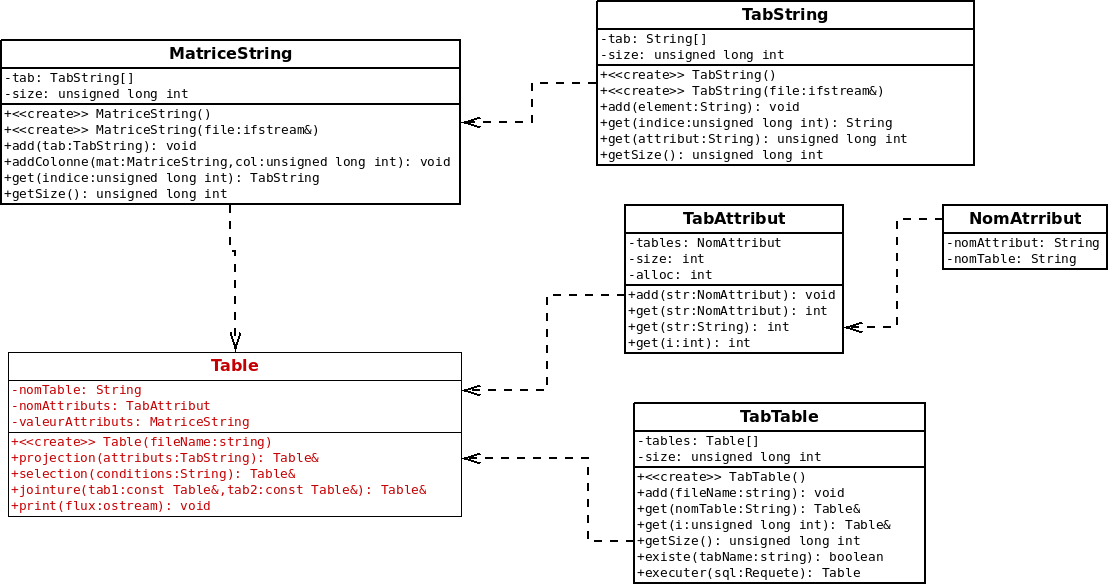
\includegraphics[width=1\textwidth]{img/sql.png}\par
	\vspace{0.1cm}
	\caption{Diagramme UML des données}
	\label{uml-donnees}
\end{figure}

\pagebreak

Nous avons choisis de modéliser notre structure de données, en utilisant l'approche orientée objet qui est parfaitement adaptée à notre problème. En effet, utiliser cette approche nous a permis de découper notre structure de données en plusieurs classes\footnote{Une classe regroupe des membres, méthodes et propriétés (attributs) communs à un ensemble d'objets.}.

La classe principale de notre application est la classe \textit{Table}.
Comme vous pouvez le voir sur le diagramme UML ci-dessus, la classe est constituée de trois attributs.

Le premier est une chaîne de caractères dans laquelle on stock le nom de la table. Cet attribut est indispensable pour identifier la table sur laquelle on veut extraire les< informations qu'on cherche.


Le deuxième attribut est une classe qui représente un tableau de chaînes de caractères dans lequel chaque case (cellule) stockera le nom de la colonne (Attribut) concernée. Il s'agit de la classe \textit{TabAttribut} qui est elle-même composée de plusieurs instances de la classe \textit{NomAttribut}.
On a représenté cette dernière comme étant le nom de l'attribut ainsi que le nom de la table d'où il provient, car cela facilitera grandement l'accès aux attributs lors de l'exécution de la requête. Ce choix sera expliqué plus en détail dans ce qui suivra.

Quant au troisième attribut, instance de \textit{MatriceString}, c'est une matrice à deux dimensions qui se chargera de stocker les valeurs de notre table.
\textit{MatriceString} est une classe constituée d'un tableau d'objets de la classe \textit{TabString} qui elle-même modélise une ligne d'une table. Tout ce mécanisme a pour effet de produire du code facilement et cela rend donc sa lisibilité, son utilisation et sa maintenance beaucoup plus facile.

La classe \textit{Table} sert donc à stocker le contenu d'un fichier. Mais cela n'est pas suffisant puisque nous serons amenés à manipuler plusieurs fichiers, alors on a pensé à rajouter la classe \textit{TabTable} pour pouvoir stocker plusieurs objets de la classe \textit{Table}, facilitant ainsi leurs manipulations.

\section{Structre de la requête}
\label{requete}
Aprés avoir modélisé la manière dont les données seront stockées, il faut à présent concevoir la façon dont la requête doit être interprétée.

Pour celà, nous avons conçu le diagramme suivant :

\vfill

\begin{figure}[!h]
	\centering
	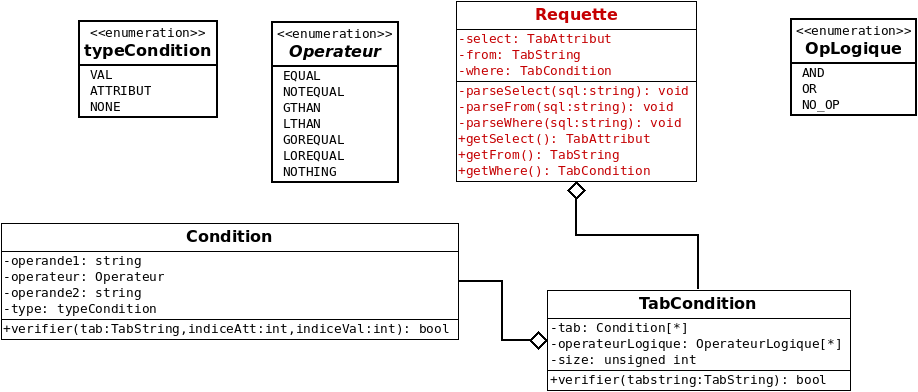
\includegraphics[width=1\textwidth]{img/requette.png}
	\vspace{0.1cm}
	\caption{Diagramme UML de la requête}
\end{figure}

\pagebreak

La structure d'une requête SQL simple est de la forme suivante : \\
\\SELECT Attribut1,Attribut2,...,AttributN\\FROM Table1,Table2,...,TableN\\WHERE condition1 [AND \textbar~OR] condition2 [AND \textbar~OR] ..... [AND \textbar~OR] conditionN;\\

Tels que \textit{Attribut1,Attribut2,...,AttributN} sont des noms d'attribut qui peuvent être considères comme des instances de la classe \textit{NomAttribut}.

\textit{Table1,Table2,...,TableN} peuvent être considérées comme des chaînes de caractères.

Et enfin, \textit{condition1 [AND \textbar~OR] condition2 [AND \textbar~OR] ..... conditionN}, qui sont des conditions
qui ont une forme un peu plus complexe, leur structure sera détaillée  plus loin dans ce chapitre.

En définissant la requête de cette façon, il est clair qu'elle peut être découpée en trois parties. En prenant en compte cette information, nous avons donc conçu la classe \textit{Requete} dans laquelle on stocke la requête SQL donnée par l'utilisateur. Cette dernière est composée de :

\subsubsection{Select}

Un attribut de la classe \textit{TabAttribut} qui contient l'ensemble des éléments à projeter. Cette classe est composée de plusieurs objets de la classe \textit{NomAttribut} qui permet de gérer les deux types de projection. c'est-à-dire, celle où seulement le nom de l'attribut est mentionné et celle où le nom de la table d'où cet attribut provient est également mentionné .

\begin{itemize}
	\item \enquote{SELECT NomAttribut ...}
	\item \enquote{SELECT NomTable.NomAttribut ...}
\end{itemize}

\subsubsection{From}

La partie \textit{From} est constituée de noms de table séparés par des virgules. Il est donc naturel, vu la simplicité, d'utiliser la classe \textit{TabString} définie plus haut.

\nb La définition d'alias pour le nom des tables n'est pas prise en charge.

\subsubsection{Where}

Enfin la dernière partie, celle qui nous a posé le plus de difficultés, est la partie \textit{Where}. Cette dernière, étant un peu plus complexe que les autres parties ; elle nous a pris un peu plus de temps pour la modéliser.

En effet, cette partie est constituée de conditions séparées par des opérateurs logiques (i.e \textit{AND} ou \textit{OR}). Telle que chaque condition est, elle même constituée de deux opérandes séparés par un opérateur arithmétique.

Nous avons donc décidé de créer deux nouvelles classes, \textit{Condition} et \textit{TabCondition}. La première est une classe qui représente une condition, c'est-à-dire deux opérandes et un opérateur. On a de même rajouté un attribut \textit{typeCondition} car une condition se découpe en deux type :
\begin{description}
	\item[Attribut - Valeur] e premier opérande étant le nom d'un attribut et le deuxième une valeur. Les valeurs prises en charge sont les suivantes : nombre réel, chaîne de caractères et date.
	\item[Attribut - Attribut] les deux opérandes sont des noms d'attribut. Cette condition est, dans la majorité des cas, utilisée pour réaliser des jointures, appelées aussi \textit{condition de jointure}
\end{description}

Pour la deuxième classe, \textit{TabCondition}, est construite à partir d'une ou plusieurs instances de la classe \textit{Condition}, ainsi que des opérateurs logiques qui les séparent.


% ------------------------------------- %
% Implementation
% ------------------------------------- %

\chapter{Implémentation}

\section{Choix de la téchnologie}
Nous avons choisis d'implémenter l'application en langage de programmation \textit{C++} parce que c'est un langage orienté objet qui est particulièrement adapté à la modélisation que nous avons précédemment réalisée. Le \textit{C++} est multiplateforme, ce qui nous permettra de porter l'application sur plusieurs systèmes, relativement facilement.

Par ailleurs, le \textit{C++} est l'un des principaux langages enseignés dans notre formation. Nous possédons donc des acquis avec ce langage, et ce projet nous permet d'en améliorer nos connaissances. Aussi ce langage regroupe une importante communauté, jouit de nombreuses bibliothèques ainsi que d'une considérable documentation.

En outre, pour la compilation du code source nous avons utilisé \textit{Make}\footnote{Make est un logiciel qui construit automatiquement des fichiers, souvent exécutables, ou des bibliothèques à partir d'éléments de base tels que du code source}. Cela nous a permis d'automatiser la production de l'exécutable.

\section{Développement}

Tout comme la partie conception, nous avons décidé de répartir l'implémentation du projet en trois parties principales.

\subsection{Chargement des données}

Nous avons commencé par implémenter les classes que nous avions modélisées dans la première partie de la conception, puis nous nous sommes concentrés sur la manière de charger le contenu d'un fichier CSV en mémoire.

La principale difficulté dans cette partie était de trouver un moyen d'interpréter un fichier CSV afin de stocker les données dans nos classes. Pour cela nous avons écrit une fonction,\textit{strsplit}, qui se charge de segmenter une ligne du fichier en plusieurs chaîne de caractères, correspondant aux valeurs ou aux noms d'attribut.

\textit{strsplit} prend en paramètre une ligne d'un fichier CSV et un caractère séparateur, une virgule par default, et retourne un tableau de chaînes de caractères qui contient les différentes valeurs. Cette fonction commence par chercher tous les caractères séparateurs qui ne sont pas libres (contenu entre des guillemets ' " '), afin d'allouer de l'espace mémoire pour stocker le résultat.
Ensuite vient la lecture des attributs. Durant cette étape, deux cas de figure se présentent, un attribut peut, ou ne pas être entouré par deux guillemets. Dans le cas où l'attribut est encadré, la fonction trouvedonc au début un guillemet et se met donc à chercher le guillemet fermant associé (qui n'est pas échapé). Et elle insère dans le tableau ce qui existe entre les deux guillemets, à la case correspondante, en utilisant la méthode \textit{substr} appartenant à la classe \textit{String} qui soustrait, dans notre cas, une chaîne de la ligne débutant par la position du guillemet ouvrant au guillemet fermant sans les prendre au compte. Dans le deuxième cas, la lecture des attributs fonctionne de la même façon mais au lieu de chercher le guillemet fermant, elle cherche le caractère séparateur.

Maintenant qu'on peut parser, on commence par lire la première ligne du fichier CSV et la passer à la fonction \textit{strsplit} en stockant le resultat dans l'attribut \textit{nomAttributs} de la classe \textit{Table} (Voir Schéma \ref{uml-donnees} page \pageref{uml-donnees}). Pour le reste du fichier, on passe chaque ligne à la fonction \textit{strsplit} et on ajoute le resultat dans la matrice \textit{valeursAttributs} de la classe \textit{Table}.

À cette étape les données sont chargées en mémoire.

\subsection{Requête}

D'abord avant de parler de l'exécution de la requête, on va expliquer comment on a interpréter cette dernière.

\subsubsection{Intérpretation}

Nous avons commencé par implémenter les classes que nous avions modélisées dans la deuxième partie de la conception (voir Chapitre \ref{requete} page \pageref{requete}), puis nous nous sommes occupés à trouver une manière de découper la requête afin de stocker chaque partie dans l'attribut correspondant.
\\
La classe \textit{requete} est constituée de trois attributs comme on l'a vu, son constructeur qui prend une chaine de caractères en argument la parse par l’utilisation des trois méthodes \textit{parseSelect(string)}, \textit{parseFrom(string)} et \textit{parseWhere(string)}, Ces trois méthodes font presque le même travail, telle que chaque méthode cherche le mot clé pour parser la requête et mettre ce qu'il faut dans l'attribut correspondant de la classe.
\\
Prenons la méthode \textit{parseSelect(string)} comme exemple. Elle prend en paramètre la requête et cherche le mot clé \textit{select} et \textit{from} pour récupérer la sous-chaîne entre ces deux mots clés qui est à son tour transformée en une instance de la classe \textit{tabAttribut} après l'avoir découpée avec la fonction  \textit{strsplit}. Et par ce même concept on obtiendra l'attribut \textit{from} et \textit{where}.

\subsubsection{Éxecution}
Maintenant on va parler de l'exécution de la requête, ce qui veut dire comment notre application va-t-elle exécuter la requête SQL sur les données qu'on a déjà chargées en mémoire vive ?
\\
Notre application exécute la requête en trois étapes consécutives et complémentaires pour effectuer le traitement nécessaire. Nous allons considérer un exemple de requête ainsi que deux tables de données afin de voir étape par étape le résultat de chaque traitement.

Exemple de requête :
\begin{center}
	\enquote{SELECT nom,localisation FROM Employés,Départements WHERE Employés.idDep = Départements.idDep AND age $\leq$ 30;}
	\begin{figure}[h]
		\begin{minipage}[c]{.46\linewidth}
			\centering
			\caption{Table 'Employés'}
			\begin{tabular}{|l|c|c|r|}
				\hline
				id & nom  & age & idDep
				\\
				\hline
				01 & Emp1 & 30  & 01    \\
				02 & Emp2 & 31  & 01    \\
				03 & Emp3 & 29  & 02    \\
				\hline
			\end{tabular}
		\end{minipage}
		\hfill%
		\begin{minipage}[c]{.46\linewidth}
			\centering
			\caption{Table 'Départements'}
			\begin{tabular}{|l|c|c|r|}
				\hline
				idDep & nom  & localisation
				\\
				\hline
				01    & Dep1 & Montpellier  \\
				02    & Dep2 & Paris        \\
				\hline
			\end{tabular}
		\end{minipage}
	\end{figure}
\end{center}

Le \textbf{produit cartésien} est fait par la méthode \textit{produitCartésien(table1,table2)} qui prend en paramètres deux tables et produit une nouvelle table en sortie. Cette table a pour nom \enquote{nomtable1 JOIN nomtable2}.Les noms d'attributs de cette table sont la concaténation des noms d'attributs des deux tables. Pour les valeurs d'attributs, chaque ligne de \textit{valeurAttributs(matrice)} de la table1 est concatenée avec toutes les lignes de \textit{valeurAttributs(matrice)} de la table2 et cela se fait par deux boucles \textit{for} imbriquées.

Le nom des tables concernées par le produit cartésien sont dans l'attribut \textit{from} de la requête. Comme on peut avoir plusieurs tables et notre méthode ne fait le produit cartésien qu'entre deux tables, on va l'effectuer entre les deux premières tables puis entre la table résultante des deux premières avec la prochaine table et ainsi de suite jusqu'à ce que le produit soit effectué entre toutes les tables.

\nb Le produit cartésien entre deux tables est une opération très couteuse en termes de mémoire vive utilisée. Notre application n'est donc pas optimisée pour les grandes tables.

À cette étape, on a une seule table résultante qui contient les attributs de toutes les tables concernées. La prochaine étape consiste à exécuter la sélection. Le résultat du produit cartésien est illustré dans la figure suivante.

\begin{center}
	\enquote{SELECT nom,localisation \textbf{FROM Employés,Départements} WHERE Employés.idDep = Départements.idDep AND age $\leq$ 30;}
	\begin{figure}[h!]
		\centering
		\caption{Execution du produit cartésien}
		\begin{tabular}{|l|c|c|c|c|c|r|}
			\hline
			id & nom  & age & Employés.idDep & Départements.idDep & nom  & localisation
			\\
			\hline
			01 & Emp1 & 30  & 01             & 01                 & Dep1 & Montpellier  \\
			02 & Emp2 & 31  & 01             & 01                 & Dep1 & Montpellier  \\
			03 & Emp3 & 29  & 02             & 01                 & Dep1 & Montpellier  \\
			01 & Emp1 & 30  & 01             & 02                 & Dep2 & Paris        \\
			02 & Emp2 & 31  & 01             & 02                 & Dep2 & Paris        \\
			03 & Emp3 & 29  & 02             & 02                 & Dep2 & Paris        \\
			\hline
		\end{tabular}
	\end{figure}
\end{center}

la \textbf{Selection} est réalisée par la méthode \textit{selection(TabCondition)} de la classe \textit{Table} qui prend en paramètre l'ensemble des conditions contenues dans l'attribut \textit{where} de la classe \textit{Requete}. La sélection est appliquée sur la table courante (la table résultante de l'étape précédente) et retourne en résultat une nouvelle table. Les noms des attributs de cette nouvelle table sont exactement les mêmes que la table courante, puisque la sélection ne concerne que les valeurs des attributs et non leurs noms.

Les valeurs d'attributs sont parcourues une par une, tout en leurs appliquant la méthode \textit{verifier} de la classe \textit{TabCondition}. Cette dernière retourne un booléen, \textit{Vrai} si les conditions, appliquées a une ligne, sont vraies et \textit{Faux} sinon. Si les conditions sont vérifier pour une ligne donnée, alors cette ligne est ajoutée à la table résultante.

Apres cette phase, on a comme résultat une table qui contient les valeurs filtrées selon les conditions de la requête. Il ne reste donc qu'à projeter les attributs que l'utilisateur a demandés . Le résultat de la sélection est schématisé ci-dessous.

\begin{center}
	\enquote{SELECT nom,localisation FROM Employés,Départements \textbf{WHERE Employés.idDep = Départements.idDep AND age $\leq$ 30};}
	\begin{figure}[h]
		\centering
		\caption{Execution de la selection}
		\begin{tabular}{|l|c|c|c|c|c|r|}
			\hline
			id & nom  & age & Employés.idDep & Départements.idDep & nom  & localisation
			\\
			\hline
			01 & Emp1 & 30  & 01 & 01 & Dep1 & Montpellier  \\
			03 & Emp3 & 29  & 02 & 02 & Dep2 & Paris        \\
			\hline
		\end{tabular}
	\end{figure}
\end{center}

La \textbf{projection} est effectuée par la méthode \textit{projection(TabAttribut)} de la classe \textit{Table} qui prend en paramètre l'ensemble des noms d'attributs que contient l'attribut \textit{select} de la classe \textit{Requete}.La projection est appliquée sur la table résultante de la sélection et retourne une nouvelle table (résultat final). Le nom des attributs de cette dernière est directement copié de l'attribut \textit{select}.La méthode se charge ensuite de copier toute les colonnes, dont le nom apparait dans l'attribut \textit{select} et de les ajouter dans la table résultante. Cette dernière est illustre ci-dessous.

\begin{center}
	\enquote{\textbf{SELECT nom,localisation} FROM Employés,Départements WHERE Employés.idDep = Départements.idDep AND age $\leq$ 30;}
	\begin{figure}[h]
		\centering
		\caption{Execution de la selection}
		\begin{tabular}{|l|r|}
			\hline
			nom  & localisation
			\\
			\hline
			Emp1 & Montpellier  \\
			Emp3 & Paris        \\
			\hline
		\end{tabular}
	\end{figure}
\end{center}

\subsection{Restitution des données}

Cette dernière étape consiste, tout bonnement, à afficher la table qui résulte de l'exécution de la requête sous deux formats simples. La première méthode est de concevoir la table dans un fichier sous un format CSV. Pour cela rien de plus simple que de parcourir la table champs par champs, les écrire tout en les entourant par des guillemets et séparant chaque champs par une virgule. Cela permet la réutilisabilité de la table pour de prochaines requêtes. La deuxième méthode consiste à retourner la table sous un format un peu plus compréhensible par un utilisateur lambda. On a donc utilisé une méthode qui écrit une table un peu comme le fait l'interpréteur de requêtes d'Oracle.
 Ci-dessous une capture d'écran d'un résultat selon cette dernière méthode.

\begin{figure}[!h]
	\centering
	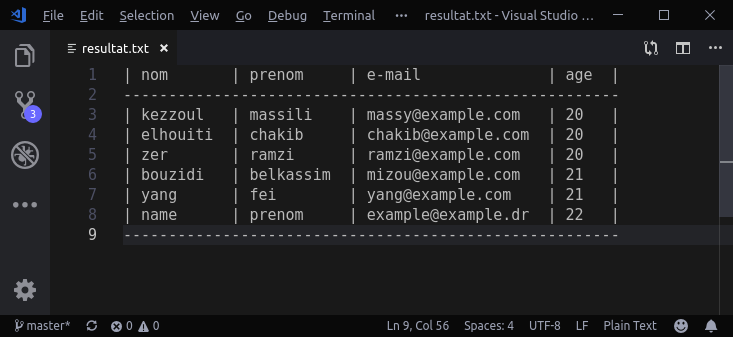
\includegraphics[width=0.65\textwidth]{img/sortie.png}
	\caption{Exemple d'une sortie de resultat}
\end{figure}

\nb Le format CSV est écrit dans le fichier \textit{resultat.csv} dans le dossier courant. Le deuxième format est quant à lui écrit dans le fichier \textit{resultat.txt} dans le dossier courant aussi.

\section{Compilation et utilisation}

\subsubsection{Compilation}

Le code source est dans le dossier \textit{src}. La compilation des sources de l'application peut se faire avec la commande suivante :

\texttt{\$ make all}

\nb la commande doit être exécutée dans le dossier où se trouve le code source.

\subsubsection{Utilisation}

Une fois le code compilé, un exécutable sera crée (\textit{sql}). Vous pourrez utiliser notre application de deux façons :

\texttt{\$ ./sql table1.csv ... tableN.csv "SELECT ... FROM ... WHERE ..."}

Les fichiers CSV sont spécifiés en argument, puis comme dernier argument, la requête SQL est entourée par des guillemets. L'application se charge de lire les fichiers et d'exécuter la requête puis d’écrire deux fichiers. Un sous le format CSV et l'autre sous un format compréhensible. Vous pourrez consulter ces fichiers grâce aux deux commande \texttt{\$ cat resultat.txt} et \texttt{\$ cat resultat.csv}. L'application s'arrête automatiquement après l'exécution et vous prévient en cas de bon déroulement ou d'erreur.

\texttt{\$ ./sql table1.csv ... tableN.csv}

En exécutant l'application de cette façon, elle charge les données en mémoire puis vous laisse la main pour donner la requête sql. Vous aurez le choix entre quatre commandes .Si votre commande commence par: \texttt{select} alors l'application considère que vous lui avez donné la requête SQL et l'exécute sur les données en mémoire. Les commandes \texttt{csv} et \texttt{txt} affichent , respectivement, le fichier \textit{resultat.csv} et \textit{resultat.txt} sur la sortie standard. Pour plus d'information, la commande \texttt{help} affiche la liste des commandes disponibles. La commande \texttt{exit} arrête l'application.

\nb Vous pourrez utiliser cette méthode sans donner aucun argument.

\section{Test}

Pour le bon déroulement de la partie implémentation, nous avons à chaque étape de développement écrit plusieurs fichiers de test. Ces fichiers consistaient à tester les modules de l'application séparément après chaque étape. Tous ces fichiers sources sont regroupés dans le dossier \textit{test} du dossier \textit{src}. Par exemple, le fichier \textit{test-condition.cpp} test la classe \textit{Condition} séparément des autres classes afin de chercher d'éventuels bogues et de veiller à son bon fonctionnement.

% ------------------------------------- %
% Bilan et difficultés rencontrées
% ------------------------------------- %

\chapter{Bilan et difficultés rencontrées}
\section{Bilan}

Au final la conception et le développement d'un moteur d'évaluation de requêtes SQL simple en mémoire vive ont pu être menés à terme et le cahier des charges respecté. Sur un plan général, ce projet nous servira comme l'un de notre premier travail en groupe autours du développement d’une application informatique. L'atteinte de l'objectif nous a permis de mieux apprécier le sens de la rigueur et du sérieux et surtout appris à nous organiser. L'organisation fut donc le plus grand enrichissement que nous ayons pu avoir.
\newline Ce projet a aussi permis de créer de vrais liens d'amitié au sein de notre groupe.

\section{Difficultés}

Plusieurs retouches ont été apportées lors de l'implémentation de notre projet, ceci est dû à des bugs. Nous sommes donc revenus sur de nombreux points de conception :
\begin{itemize}
	\item
\end{itemize}
% ------------------------------------- %
% Perspective
% ------------------------------------- %

\chapter{Perspective}

Dans une vision d'amélioration de notre application voici quelques idées sur lesquelles nous avons réfléchi :

\subsubsection{Optimisation}

Une optimisation en mémoire de notre application semble l'une des premières perspectives sur laquelle nous devons nous pencher. En effet, notre application ne permet pas d'exécuter des jointures entre des tables assez conséquentes. Afin d'optimiser cela, plusieurs solutions sont possibles.

\begin{itemize}
	\item Commencer par l'exécution d'une projection partielle. C'est-à-dire supprimer les attributs (colonnes) qui n'apparaissent pas sur les conditions de sélection. Cela réduira, grandement dans certains cas, la taille des tables sur laquelle la jointure sera exécutées.
	\item Ensuite, dans la même optique de réduction de la taille des tables, exécuter les conditions de sélection (hors conditions de jointure) sur chaque tables individuellement.
	\item Enfin, après toutes ces manipulations, il est envisageable d'écrire le résultat du produit cartésien dans un fichier temporaire et pas directement en mémoire, afin de ne jamais surcharger la mémoire vive. Mais cela entraînera, en contre partie, un temps d'exécution plus longs.
\end{itemize}

\subsubsection{Opérateur}

Il est aussi possible d'ajouter certains opérateurs à notre selection telles que :
\begin{description}
	\item[LIKE] Ce mot-clé permet d’effectuer une recherche sur un modèle particulier. Il est par exemple possible de rechercher les enregistrements dont la valeur d’une colonne commence par telle ou telle lettre.
	\item[BETWEEN] Permet de sélectionner un intervalle de données dans une requête.
	\item[IN] L’opérateur logique qui vérifie si une colonne est égale à une des valeurs comprises dans set de valeurs déterminées.
\end{description}

\subsubsection{Commandes}

Ajouter des commandes en plus autre que \textit{SELECT, FROM} et \textit{WHERE}.

\begin{description}
	\item[GROUP BY] qui est utilisée en SQL pour grouper plusieurs résultats et utiliser une fonction de totaux sur un groupe de résultat. Sur une table qui contient toutes les ventes d’un magasin, il est par exemple possible de regrouper les ventes par clients identiques et d’obtenir le coût total des achats pour chaque client.
	\item[HAVING] condition qui, en SQL, est presque similaire à WHERE à la seule différence que HAVING permet de filtrer en utilisant des fonctions telles que SUM(), COUNT(), AVG(), MIN() ou MAX().
	\item[AS] permet d’utiliser des alias pour renommer temporairement une colonne ou une table dans une requête. Cette astuce est particulièrement utile pour faciliter la lecture des requêtes et indispensable dans certaines requête imbriquées.
\end{description}

\subsubsection{Fonctions d'agrégation}

Nous avons aussi pensé à rajouter des fonctions d'agrégation, mais le temps ne nous l'a pas permis.

\begin{description}
	\item[MAX()/MIN()] Fonction qui calcul la valeur maximal/minimal d'un attribut.
	\item[COUNT()] Fonction qui calcul le nombre de ligne de la table resultat.
	\item[SUM()] Fonction qui a calcul la somme des valeurs d'un attribut.
	\item[AVG()] Fonction qui calcul la moyenne des valeurs d'un attribut donné.
\end{description}

% ------------------------------------- %
% Annexes
% ------------------------------------- %

\appendix

\chapter{Annexes}


\end{document}
